\documentclass[]{article}
\usepackage[utf8]{inputenc}
\usepackage[italian]{babel}
\usepackage{amsmath}
\usepackage{amssymb}
\usepackage{graphicx}
\usepackage{listings}
\usepackage{color}
\begin{document}
\newcommand{\campo}[1]{\mathbb{#1}}

\definecolor{LightLightGray}{RGB}{241,241,241}
\lstset{
belowcaptionskip=1\baselineskip,
 breaklines=true,
 frame=L,
 xleftmargin=\parindent,
 language=C,
 showstringspaces=false,
 basicstyle=\footnotesize\ttfamily,
 keywordstyle=\bfseries\color{green!40!black},
 commentstyle=\itshape\color{purple!40!black},
 identifierstyle=\color{blue},
 stringstyle=\color{orange},
}

\title{Relazione sull'implementazione del simulatore biologico WATOR}
\author{Alessandro Pagiaro}
\date{\today}
\maketitle
\tableofcontents
\clearpage

\section{Il processo principale: Wator}
Il processo Wator rappresenta il nucleo operativo di tutto il programma. Il processo è suddiviso in vari thread:
\begin{itemize}
	\item Main Thread
	\item Dispatcher
	\item Collector
	\item Signal Handler
	\item Worker$_1$, .., Worker$_n$
\end{itemize}

\subsection{Schema Grafico}
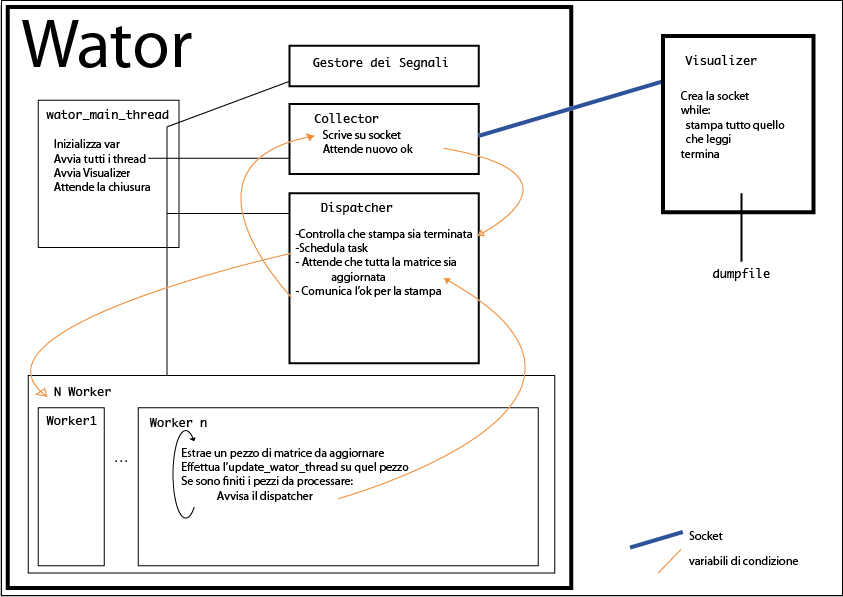
\includegraphics[width=400pt]{wator.png}

\subsection{Main Thread (wator\_main\_thread.c)}
Il \texttt{wator\_main\_thread.c} è il thread che si preoccupa di avvia il processo completo. All'avvio esegue in ordine le seguenti operazioni:
\begin{itemize}
	\item Inizializza tutte le variabili interi, le mutex e le condition
	\item Verifica che esiste la directory per la creazione della socket e che non contenga una precedente socket creando poi problemi di creazione della nuova
	\item Maschera tutti i segnali rilevanti per il processo (verrà approfondito nella sezione Signal Handler)
	\item Legge le opzioni passate all'avvio e ne verifica la validità
	\item Prova ad avviare i thread necessari all'esecuzione del processo:
		\begin{itemize}
			\item Prova ad avviare il \texttt{Signal Handler}
			\item Prova ad avviare $n$ thread \texttt{Worker}
			\item Prova ad avviare il thread \texttt{Collector}
			\item Prova ad avviare il thread \texttt{Dispatcher}
			\item Prova ad avviare il processo \texttt{Visualizer}
		\end{itemize}
	\item Si mette in attesa sui thread avviati
	\item Al termine dei vari thread, distrugge le mutex e le variabili di condizione
	\item Termina
\end{itemize}
All'avvio dei vari thread viene verifica l'avvenuta creazione. In caso in cui questa fallisca si è deciso di ritentare per un numero di volte pari a \texttt{MAX\_TRY}, attendendo un numero esponenziale di secondi ad ogni nuovo tentativo. 

\subsection{Thread Dispatcher (dispatcher.c)}
Il thread \texttt{Dispatcher} è colui che si preoccupa di schedulare i vari thread e di azzerare le variabili di supporto alla simulazione ad ogni chronon. \\
Effettua in ordine le seguenti operazioni:
\begin{itemize}
	\item Alloca la matrice \texttt{skip}, usata dalla funzione $update$.
	\item Inizia la fase di aggiornamento:
		\begin{itemize}
			\item Azzera la matrice \texttt{skip}
			\item Si assicura che il \texttt{Collector} abbia terminato la stampa prima di procedere
			\item Mette a disposizione dei thread \texttt{Worker} le Sottomatrici da aggiornare
			\item Attende che l'aggiornamento sia completato
			\item Se sono passati \texttt{intervallo\_di\_stampa} chronon, comunica al \texttt{Collector} di inviare la stampa
		\end{itemize}
	\end{itemize}
Nel caso in cui Il \texttt{Collector} stia stampando, e quindi il \texttt{Dispatcher} non può procedere alla stampa altrimenti c'è il rischio di aggiornare la matrice durante la stampa, il \texttt{Dispatcher} si mette in attesa sulla variabile di condizione \texttt{stampa\_effettuata}. Per la sincronizzazione viene quindi usata la mutex \texttt{stampa\_mux}. \\
Per la sincronizzazione tra gli $n$ thread \texttt{Worker}, che estraggono dalla lista delle Sottomatrici, e il thread \texttt{Dispatcher}, che invece inserisce elementi nella lista delle Sottomatrici, viene usata la mutex \texttt{lista\_mux}.

Il thread \texttt{Dispatcher} prima di effettuare la stampa si assicura che:
\begin{itemize}
	\item La lista delle Sottomatrici sia vuota, cioè che i \texttt{Worker} abbiano estratto tutti gli elementi
	\item Il \texttt{count\_worker} sia uguale a 0, cioè che non ci sono \texttt{Worker} che stanno effettuando l'$update$ della sottomatrice.
\end{itemize}
La variabile \texttt{count\_worker} viene incrementata ogni qual volta la funzione $extract$ chiamata da un \texttt{Worker} riesce ad estrarre un elemento dalla lista delle Sottomatrici (\texttt{lista\_pezzi}) e viene decrementata dal \texttt{Worker} quando la funzione $update$ termina.

\subsection{Thread Collector (collector.c)}
Il thread \texttt{Collector} è colui che si preoccupa di mandare le informazioni da stampare al processo \texttt{Visualizer}.\\
All'avvio tenta di connettersi alla socket \texttt{SOCKNAME} che viene creata dal \texttt{Visualizer}. Qualora la socket non esista ancora, e quindi la funzione $connect$ restituisce l'errore ENOENT, si addormenta per 250 millisecondi e ritenta.\\
Connesso quindi alla socket effettua ciclicamente (finché non viene settata la variabile di chiusura dal thread \texttt{Dispatcher}) le seguenti operazioni:
\begin{itemize}
	\item Controlla se può stampare o deve attendere il Dispatcher
	\item Scrive sulla socket la lettera \texttt{A}, token che per convenzione determina l'inizio di una nuova matrice, permettendo al \texttt{Visualizer} quando termina la stampa di una matrice e ne inizia una nuova
	\item Scrive sulla socket la matrice completa
	\item Setta la variabile \texttt{puoi\_procedere} a \textbf{true} e risveglia eventualmente il thread \texttt{Dispatcher} in attesa sulla variabile di condizione \texttt{stampa\_effettuata}.
	\item Si sospende sulla variabile di condizione \texttt{stampa\_pronta} finché non ritorna \textbf{true} la variabile \texttt{puoi\_stampare}.
\end{itemize}

Al comando di chiusura, quando cioè la variabile \texttt{close\_all} viene settata a \textbf{true} dal \texttt{Gestiore Segnali}, viene chiusa la socket facendo terminare anche il processo \texttt{Visualizer} (come approfondito nella sezione \texttt{Visualizer}).

\subsection{Thread Worker (worker.c)}
Il thread \texttt{Worker} è il thread che effettivamente aggiorna la matrice chiamando al suo interno la funzione $update$. Questo effettua una corsa critica con gli altri $n-1$ thread \texttt{Worker} per estrarre dalla lista delle Sottomatrici \texttt{lista\_pezzi} la sottomatrice da aggiornare.\\
Il thread \texttt{Worker} effettua ciclicamente le seguenti operazioni:
\begin{itemize}
	\item Estrae la sottomatrice tramite la funzione $extract$ (che sospende il thread in caso in cui la lista \texttt{lista\_pezzi} sia vuota)
	\item Preleva dall'elemento estratto solo le informazioni riguardante le informazioni della sottomatrice, liberando la memoria in eccesso
	\item Effettua $update$ sulla sottomatrice
	\item Verifica che non ci siano altri pezzi da elaborare e che non ci siano altri \texttt{Worker} a lavoro. Se entrambe le condizioni sono vere:
		\begin{itemize}
			\item Controlla che non è richiesta la terminazione della simulazione
			\item Sveglia, se necessario, il thread \texttt{Dispatcher} inviando un segnale alla variabile di condizione \texttt{stanno\_lavorando}
		\end{itemize}
	\end{itemize}
I controlli finali sono effettuati accedendo in mutua esclusione sia con gli altri thread \texttt{Worker} sia con il thread \texttt{Dispatcher}. 
\subsection{Gestore Segnali (gestione\_segnali.c)}
Il thread \texttt{Gestione Segnali} è colui che si preoccupa di ricevere i segnali inviati al processo e gestirli opportunamente, settando le giuste variabili globali interpretate poi dai vari thread.\\
Tutti i thread, infatti, hanno i segnali relativi al processo mascherati. \\
\subsubsection{Il segnali di \texttt{SIGINT} o di \texttt{SIGTERM}}
Questi due segnali richiedono l'esecuzione gentile del processo. Registrati dal thread \texttt{Gestore Segnali}, viene settata a \textbf{true} la variabile \texttt{close\_all} che farà uscire dal ciclo computazionale i thread \texttt{Dispatcher} e \texttt{Collector}.\\ \\
Per effettuare la chiusura gentile, cioè per terminare l'aggiornamento della matrice e stampare l'ultimo stato, il thread \texttt{Dispatcher} controlla la variabile solo al termine di un'aggiornamento. Uscito quindi dal ciclo di aggiornamento setta a \textbf{true} la variabile \texttt{termine\_elaborazione} che comunica ai thread \texttt{Worker} che il \texttt{Dispatcher} è terminato e quindi devono a loro volta terminare. I thread \texttt{Worker} non possono usare direttamente direttamente la variabile \texttt{close\_all} poichè non è detto che tutta la lista delle Sottomatrici sia stata aggiornata e controllano quindi la variabile \texttt{termine\_elaborazione} per terminare la loro esecuzione.\\

Per assicurarsi che tutti i thread \texttt{Worker} possano valutare la condizione di terminazione, viene inviata una $broadcast$ per portare nella lista pronti tutti quelli in attesa. Situazione analoga viene realizzata con il thread \texttt{Collector} effettuando una $signal$ sulla variabile \texttt{stampa\_pronta} \\ 

Al termine dell'esecuzione il thread \texttt{Dispatcher} invia un ultimo segnale di stampa al \texttt{Collector} il quale effettuerà un'ultimo ciclo di stampa e terminerà poichè la variabile \texttt{termine\_esecuzione} sarà stata messa a \textbf{true}. 

\subsubsection{Il segnale \texttt{SIGUSR1}}
Questo segnale comunica al processo di dover stampare il wator.check. Questa funzione, a differenza della classica stampa della matrice sul \texttt{dumpfile}, viene effettuata dal thread \texttt{Dispatcher}. Questo poichè il thread \texttt{Collector} viene risvegliato dall'attesa solo ogni \texttt{intervallo\_di\_stampa} chronon, non potendo quindi assicurare una stampa  del \texttt{wator.check} nel chronon in cui viene richiesta.


\section{Il processo di stampa: Visualizer}
Questo processo non fa altro che creare la socket \texttt{SOCKNAME}, valutare il parametro che gli è stato passato \texttt{dumpfile} e quindi leggere finchè non viene chiusa la socket dallo scrittore \texttt{Collector} stampando quel che legge sul \texttt{dumpfile}.\\
Qualora \texttt{dumpfile} è lo \texttt{stdout} la stampa avviene come stream, altrimenti il file \texttt{dumpfile} contiene solamente l'ultimo aggiornamento della matrice pianeta.

\section{Funzioni Rilevanti}
\subsection{split\_matrice}
Questa funzione, dichiarata nel file \texttt{wator\_thread\_funzioni}, si occupa di dividere la matrice del pianeta in varie sottomatrici che saranno poi aggiunte (sottoforma di puntatori) alla lista \texttt{lista\_pezzi} dal \texttt{Dispatcher} ed estratte dagli $n$ \texttt{Worker}.
Questa funzione divide la matrice in tanti quadranti di dimensione \texttt{K} e \texttt{N}, settati da opportuna macro. Qualora la matrice ha un avanzo crea dei rettangoli di dimensioni degli elementi rimanenti.

\subsection{update\_wator\_thread}
È la funzione di aggiornamento della sottomatrice di competenza. Viene invocata dal thread \texttt{Worker}.\\
La funzione esegue un'aggiornamento lineare sulla sottomatrice accedendo alle aree critiche (le prime/ultime due righe/colonne) tramite mutex unica.
Le celle critiche sono chiaramente quelle che confinano (che definiamo critiche$_1$) con altre sottomatrici per ovvie ragione ma anche quelle più interne, cioè quelle sulla seconda riga, sulla seconda colonna, sulla penultima riga e penultima colonna (critiche$_2$), poichè un eventuale animale potrebbe spostarsi capitando su su una cella critica$_1$ che in quel momento è acceduta anche dal thread \texttt{Worker} adiacente.
\subsection{add}
La funzione $add$ è quella che gestisce l'inserimento delle sottomatrici in una lista. Accede alla lista in mutua esclusione. Dopo aver inserito un elemento effettua una $signal$ sulla variabile di condizione \texttt{lista\_vuota} in modo da mettere nello stato di pronto un eventuale thread \texttt{Worker} in attesa.
\subsection{extract}
La funzione $extract$ è quella che gestisce l'estrazione degli elementi dalla lista delle sottomatrici. È invocata dai thread \texttt{Worker}. Nel caso in cui la lista sia vuota mette il thread in attesa sulla variabile di condizione \texttt{lista\_vuota}.
\section{Lo script bash Watorscript}
Lo script \texttt{Watorscript} è uno script di supporto al simulatore. Verifica la correttezza sintattica del pianeta, ne conta il numero di squali e di pesci. \\
Il $parsing$ delle opzioni avviene mediante l'utility \texttt{getopt}. 

\section{Installazione}
Per l'installazione si può ricorrere all'utility \texttt{Make}. Basterà invocare il comando \texttt{make install} o alternativamente \texttt{make wator; make visualizer}.
\section{Mappa dei file del progetto}
\section{File Sorgenti}
\begin{itemize}
	\item wator\_thread\_funzioni.h
	\begin{itemize}
		\item wator\_thread\_funzioni.c
		\item dispatcher.c
		\item collector.c
		\item worker.c
		\item gestore\_segnali.c
		\item wator\_main\_thread.c
	\end{itemize} 
	\item valutazione\_argomenti.h
	\begin{itemize}
		\item valutazione\_argomenti.c
	\end{itemize}
	\item wator.h
	\begin{itemize}
		\item wator.c
	\end{itemize}
	\item Visualizer.c
\end{itemize}
\end{document}